Describes which method has been used in the attempt to classify North Atlantic Right Whales from images.

\subsection{Classification Algorithm}
Also known as \emph{Supervised Learning Algorithm}
Describes which algorithm was used to classify North Atlantic Right Whales. Classification Algorithms have one thing in common, which is that they require data input to be on a similar data structure.
The overall data structure for classifications is that it can contain 1..n observations which each has x amount of data points. For a model, the amount of data points for each observation has to be the same. An example as seen in Table \ref{tab:example data} shows how data could look.
If an observation is missing a value, it can be set to NA\footnote{Not Available} instead. It still has to be present in the structure.

\begin{table}
  \centering
  \caption{Example data}
  \label{tab:example data}
  \begin{tabularx}{\linewidth}{|l|X|X|X|X|} \hline
    obs. & x1 & x2 & x3 & x4 \\ \hline
    1    & 20 & 74 & 84 & 82 \\ \hline
    2    & 52 & 33 & 4  & 36 \\ \hline
    3    & 78 & 55 & 57 & 3  \\ \hline
    4    & 61 & 68 & 65 & 5  \\ \hline
  \end{tabularx}
\end{table}

\subsubsection{Decision Tree}
Decision tree is a classification algorithm. 
A decision is a binary tree structure where the path in each node is decided based on a split on a given input variable.
This variable split is configured to limit the amount of possible classes down each path. This is done by calculating the entropy (information gain) on each split on a given input variable/feature. This is then done for all input variable. A higher information gain means that a certain split separates different classes better.  
At the end of a path, a leaf contains the class to represent that exact path.
When prediction against a decision tree that leaf is given as the returned prediction.

\subsubsection{Random Forest}
Random Forest is an algorithm which is based upon the decision trees and wisdom of the crowd.
Random Forest spawn multiple decision trees, the algorithm for splitting in the decisions tree in random forest does however differs from how it is done in normal decisions trees.
Random Forest use ``feature bagging'' at each node and then decide for the splitting feature on that subset rather than all the features. This ensures that decision trees isn't identical, but offers variety.

\subsubsection{Neural Network}
Neural Networks is an algorithm as an attempt to mimic how human learns.
Neural Networks do however variate from how neurons and connections works in the brain as it contains a link from each node in layer x to each node in layer x + 1. As seen at Figure \ref{fig:neuralnetwork}, a neural network with only a input layer and a output layer is shown and the connections between the nodes. Each input node in the figure is connected to all the output nodes.

\begin{figure}
  \centering
  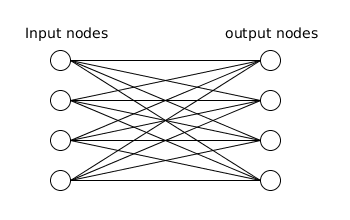
\includegraphics[width=0.7\linewidth]{Images/neuralnetwork}
  \caption{Neural Network with no hidden layers}
  \label{fig:neuralnetwork}
\end{figure}

\subsection{Clustering}
Is an \emph{Unsupervised Learning Algorithm} and was used for the preprocessing of the dataset. The specific implementation of the clustering used was K-Means. It splits the data into n clusters and uses euclidean distance to calculate which cluster to add new observations to. Every time new data is added, the center of the clusters are recalculated.